
\documentclass{article} % For LaTeX2e
\usepackage{iclr2025_conference,times}

\input{math_commands.tex}

\usepackage{hyperref}
\usepackage{url}
\usepackage{graphicx}
\usepackage{booktabs}
\usepackage{multirow}

\title{Domain-Adaptive Embedding Fine-Tuning for Financial Retrieval in RAG Systems}

\author{Jiaqi Deng, Hongbin Zhong}

\newcommand{\fix}{\marginpar{FIX}}
\newcommand{\new}{\marginpar{NEW}}

\iclrfinalcopy
\begin{document}

\maketitle

\begin{abstract}
Retrieval-augmented generation (RAG) systems depend on retrieval quality, yet general-purpose embedding models often underperform on domain-specific corpora where relevance hinges on specialized terminology and implicit semantic distinctions.
We investigate domain-adaptive fine-tuning of dense retrievers for financial text using BGE embedding models trained with Multiple Negatives Ranking Loss on FiQA-2018, with controlled ablations across (1) fine-tuning versus zero-shot retrieval, (2) hard negative mining, and (3) model capacity scaling from 33M to 110M parameters.
Fine-tuning \texttt{bge-small-en} (33M) raises nDCG@10 from 0.3109 to 0.3916 (+26.0\%) and Recall@10 from 0.3653 to 0.4572 (+25.1\%) on the test set.
However, the same recipe produces no observable improvement at the larger scale: fine-tuning \texttt{bge-base-en-v1.5} (110M) yields nDCG@10 of 0.4053, within measurement noise of its zero-shot baseline of 0.4062.
We observe the same qualitative pattern across four tested configurations spanning learning rate, batch size, and parallelism, which reduces concern that the result is driven by a single recipe but does not fully rule out hyperparameter sensitivity.
This reveals a capacity-dependent interaction: under small-scale fine-tuning, gains for stronger pretrained encoders may come from pretraining itself rather than from domain adaptation.
Hard negative mining without denoising further degrades performance under sparse relevance labels.
Code and trained-model evaluation logs are available at \url{https://github.com/rjzhb/DLFinalProj}.
\end{abstract}

\section{Introduction}

Dense retrieval has become a critical component of modern retrieval-augmented generation (RAG) systems, since the quality of retrieved evidence directly affects downstream response quality.
This issue is particularly pronounced in the financial domain, where relevant passages often involve specialized terminology, subtle semantic distinctions, and context-dependent language.
Consequently, general-purpose embedding models may fail to capture finance-specific notions of relevance, leading to suboptimal retrieval performance even when the overall retrieval framework is strong.

In this work, we ask: \emph{Can domain-adaptive fine-tuning of a pretrained dense retriever significantly improve retrieval quality on financial text, and how do model capacity and training strategy affect the outcome?}
Success is defined as a meaningful improvement in nDCG@10 and Recall@10 on the held-out FiQA test split over the lexical (BM25) and same-encoder zero-shot baselines.
This work benefits developers of financial RAG applications---such as investment research assistants, regulatory compliance tools, and financial QA systems---by demonstrating a lightweight adaptation strategy that improves retrieval without modifying the downstream generator.

\begin{figure}[t]
    \centering
    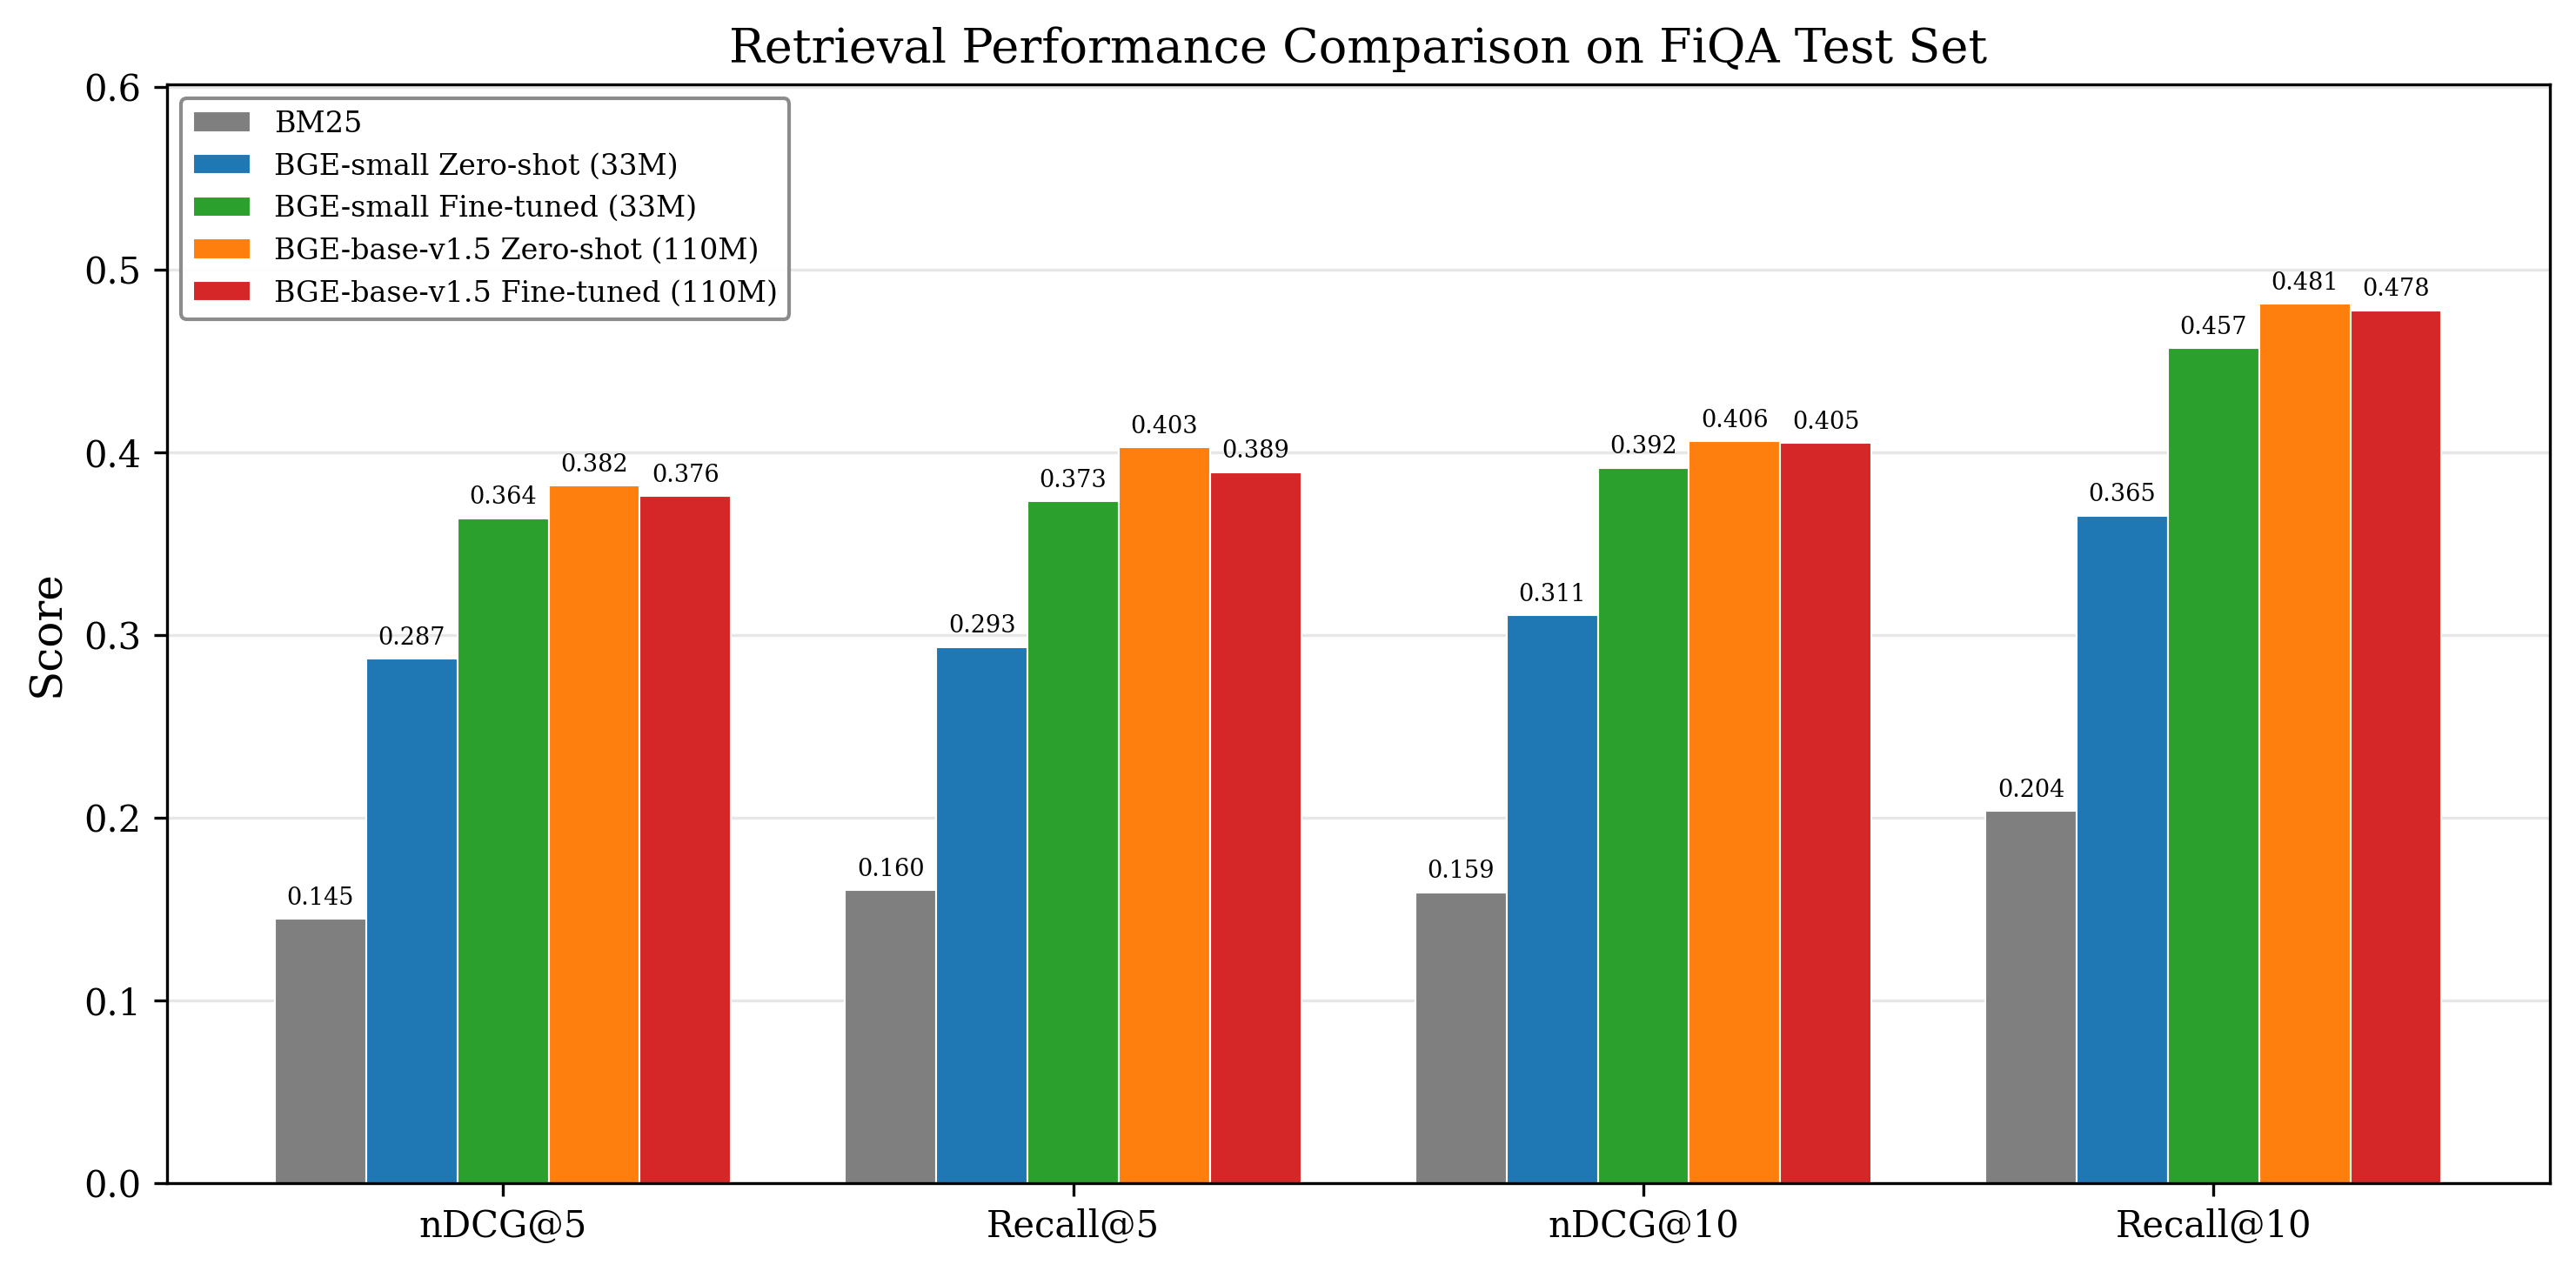
\includegraphics[width=\linewidth]{figures/comparison_all.png}
    \caption{Retrieval performance on the FiQA test set across BM25, zero-shot, and fine-tuned BGE encoders at two scales. Fine-tuning yields large gains for the small (33M) encoder but no measurable benefit for the base (110M) encoder, whose zero-shot baseline already matches the fine-tuned variant.}
    \label{fig:teaser}
\end{figure}

\section{Problem Formulation and Related Work}

\subsection{Problem Formulation}

We formulate the task as dense passage retrieval.
Given a natural-language query $q$ and a corpus of candidate passages $\mathcal{D} = \{p_1, \dots, p_N\}$, the goal is to learn a retrieval function $R(q, \mathcal{D}) \rightarrow \{p_{\pi(1)}, \dots, p_{\pi(k)}\}$ that ranks passages by semantic relevance.
A dual-encoder model maps queries and passages independently into a shared embedding space:
\[
\mathbf{v}_q = f_{\theta}(q), \qquad \mathbf{v}_p = f_{\theta}(p),
\]
where $f_{\theta}$ denotes the shared transformer encoder followed by pooling and L2 normalization.
Relevance is computed by cosine similarity: $\mathrm{sim}(q,p) = \mathbf{v}_q^\top \mathbf{v}_p$.
The input is a set of query--passage relevance pairs $\{(q_i, p_i^+)\}$ for training; the output is a ranked list of passages for each test query, evaluated against gold relevance annotations.

\subsection{Related Work}

\paragraph{Dense retrieval.}
Retrieval quality in RAG systems is critical because retrieval errors propagate downstream \citep{lewis2020retrieval}.
BM25 remains a strong lexical baseline \citep{robertson2009probabilistic}, while DPR demonstrated that dual-encoder dense retrieval can outperform lexical methods when semantic matching matters \citep{karpukhin2020dense}.
SBERT introduced efficient siamese sentence embeddings \citep{reimers2019sentence}, and BGE-style models improved retrieval through large-scale contrastive pretraining \citep{xiao2023cpack,flagembedding2023}.

\paragraph{Domain transfer and financial retrieval.}
BEIR documents weak zero-shot generalization on heterogeneous retrieval tasks \citep{thakur2021beir}, and FinMTEB shows that strong general-purpose performance does not necessarily transfer to finance \citep{tang2025finmteb}.
FiQA-2018 provides a standard benchmark for evaluating finance-domain retrieval \citep{maia201818}.

\paragraph{Hard negative mining.}
ANCE uses approximate nearest neighbor search to mine difficult negatives during training \citep{xiong2020approximate}, and RocketQA improves dual-encoder training through denoised hard negatives \citep{qu2021rocketqa}.
Our work investigates whether hard negative mining helps when the underlying relevance annotations are sparse.

\paragraph{Positioning.}
Table~\ref{tab:positioning} summarizes how our work relates to prior methods.
Our contribution is an empirical study of domain-adaptive fine-tuning for financial retrieval, with ablations across model scale, training strategy, and query conditioning that are not available in prior work on FiQA.

\begin{table}[t]
    \centering
    \scriptsize
    \begin{tabular}{lcccc}
        \toprule
        Method & Domain & Hard neg. & Model scaling & Ablation scope \\
        \midrule
        DPR \citep{karpukhin2020dense} & Open-domain QA & No & Single & Architecture \\
        ANCE \citep{xiong2020approximate} & General & ANN-mined & Single & Neg. strategy \\
        RocketQA \citep{qu2021rocketqa} & General & Denoised & Single & Neg. denoising \\
        BGE \citep{xiao2023cpack,flagembedding2023} & General & In pretrain & S/B/L & Pretraining \\
        \textbf{Ours} & \textbf{Finance} & \textbf{Ablated} & \textbf{33M/110M} & \textbf{Full pipeline} \\
        \bottomrule
    \end{tabular}
    \caption{Comparison with related approaches. Unlike prior work, we provide controlled ablations across training strategy, model scale, and query conditioning on a domain-specific financial benchmark.}
    \label{tab:positioning}
\end{table}

\section{Method}

\subsection{Hypotheses}

We test three hypotheses:

\textbf{H1:} Fine-tuning on FiQA with Multiple Negatives Ranking Loss improves nDCG@10 and Recall@10 over zero-shot dense retrieval with the same encoder. We expect this because the pretrained encoder lacks exposure to finance-specific relevance patterns.

\textbf{H2:} Adding retrieval-based hard negatives improves retrieval quality over the in-batch-negative baseline when the encoder, optimizer, and batch size are held fixed. We expect this because hard negatives force the model to distinguish semantically similar but non-relevant passages.

\textbf{H3:} Scaling model capacity from 33M parameters (\texttt{bge-small-en}) to 110M parameters (\texttt{bge-base-en-v1.5}) under the same fine-tuning protocol yields higher retrieval quality than the smaller fine-tuned model. We expect this because larger encoders capture finer-grained semantic distinctions and benefit equivalently from domain adaptation.

\subsection{Training Pipeline}

Our retriever follows a Sentence-Transformer dual-encoder architecture.
Training uses Multiple Negatives Ranking Loss (MNR):
\[
\mathcal{L}
=
-\frac{1}{n}\sum_{i=1}^{n}
\log
\frac{\exp(\mathrm{sim}(q_i, p_i^+) \cdot s)}
{\sum_{j=1}^{n}\exp(\mathrm{sim}(q_i, p_j^+) \cdot s)},
\]
where $s = 1/\tau = 20.0$ is the inverse temperature scale.
Each query is prepended with the BGE retrieval instruction prefix: \texttt{"Represent this sentence for searching relevant passages: "}, following the asymmetric retrieval protocol recommended by the BGE authors.
Passages are encoded without a prefix.

We experiment with two training stages:
\begin{itemize}
    \item \textbf{Stage 1 (in-batch negatives):} Standard MNR training with query--positive pairs, where other passages in the mini-batch serve as implicit negatives.
    \item \textbf{Stage 2 (hard negatives):} The Stage~1 checkpoint retrieves the top-50 passages for each training query; non-relevant passages among the top results are used as hard negatives, forming $(q, p^+, p^-)$ triplets for continued training at a reduced learning rate.
\end{itemize}

Model selection uses the best validation nDCG@10 across epochs, with the \texttt{save\_best\_model} flag enabled.

\subsection{Evaluation Strategy}

We evaluate all methods under a shared protocol on the FiQA test split (648 queries).
Passage embeddings are indexed with FAISS \citep{douze2025faiss} using inner-product search on L2-normalized vectors (equivalent to cosine similarity).
We report nDCG@5, nDCG@10, Recall@5, and Recall@10.

Baselines: (1) BM25 with whitespace tokenization \citep{thakur2021beir}; (2) zero-shot \texttt{bge-small-en} (33M); and (3) zero-shot \texttt{bge-base-en-v1.5} (110M).
These span lexical, small dense, and large dense retrieval. Crucially, the zero-shot baselines at both scales let us isolate the contribution of fine-tuning from the contribution of model capacity.

\subsection{Reproducibility Details}

All code, configurations, and trained-model evaluation logs are released at \url{https://github.com/rjzhb/DLFinalProj}.
Both encoders share the same training recipe: AdamW optimizer, learning rate $2\times 10^{-5}$, 10\% warmup, weight decay 0.01, MNR loss scale $20.0$, max sequence length 512, query instruction prefix enabled, and best-checkpoint selection by validation nDCG@10.
The smaller \texttt{bge-small-en} (33M, 384-dim) is trained on a single A40 GPU with batch size 64 for 5 epochs; the larger \texttt{bge-base-en-v1.5} (110M, 768-dim) is trained with DDP on four A40 GPUs at batch size 32 per GPU (effective 128) for 3 epochs.
All experiments use sentence-transformers (v5.3.0), PyTorch, FAISS-CPU, and were run on NVIDIA A40 (46 GB) GPUs on the Georgia Tech PACE cluster with the default random seed (42).
Stage~2 hard negative mining loads the best Stage~1 checkpoint, retrieves the top-50 passages per training query, treats non-relevant passages as hard negatives (up to 3 per positive), and continues training with MNR loss at $5\times 10^{-6}$ for 2 epochs.

\section{Data}

We use FiQA-2018 \citep{maia201818}, a financial opinion mining and question answering dataset from the WWW'18 Open Challenge.

\paragraph{Source and composition.}
The corpus contains 57,638 financial text passages drawn from financial microblogs, news articles, and QA forum posts.
The query set contains 6,648 natural-language questions about financial topics including investment strategy, market analysis, and personal finance.
Relevance labels are binary (relevant/not relevant) and were annotated by domain experts.

\paragraph{Data splits.}
We use the BEIR-standard partition: 5,500 training queries, 500 validation queries, and 648 test queries.
Training produces 14,166 query--positive passage pairs.
The corpus is shared across all splits.

\paragraph{Preprocessing.}
For each corpus document, we concatenate the title and body text with a space separator.
No additional cleaning, lowercasing, or stemming is applied to preserve financial terminology (e.g., ``P/E ratio'', ``10-K filing'').
Passages are tokenized by the model's WordPiece tokenizer and truncated to 512 tokens.
For BM25, we apply whitespace tokenization on lowercased text.
No data augmentation is used; duplicating pairs can create false in-batch negatives under MNR loss \citep{qu2021rocketqa}.

\paragraph{Known limitations.}
The relevance annotations are sparse---each query has on average only 2.6 labeled relevant passages out of 57,638 candidates, and many truly relevant passages remain unlabeled.
This sparsity has implications for hard negative mining, as discussed in Section~\ref{sec:hn_analysis}.
The dataset is English-only and skewed toward retail financial topics (personal finance, investment advice), with limited coverage of institutional finance or quantitative trading.

\section{Experiments and Results}

\subsection{Overall Retrieval Performance}

Table~\ref{tab:main_results} presents the main results.
Fine-tuning improves substantially over the zero-shot baseline for \texttt{bge-small-en}, but not measurably for \texttt{bge-base-en-v1.5}, so H1 holds only at the smaller scale.
The strongest absolute test scores come from \texttt{bge-base-en-v1.5} (both zero-shot and fine-tuned variants reach nDCG@10 $\approx 0.405$), but as shown in Table~\ref{tab:main_results} the fine-tuned base model does not exceed its own zero-shot baseline on the reported test metrics.

\begin{table}[t]
    \centering
    \scriptsize
    \begin{tabular}{lcccc}
        \toprule
        Model & nDCG@5 & Recall@5 & nDCG@10 & Recall@10 \\
        \midrule
        BM25 & 0.1446 & 0.1603 & 0.1591 & 0.2037 \\
        BGE-small-en (zero-shot, 33M) & 0.2870 & 0.2935 & 0.3109 & 0.3653 \\
        BGE-small-en (fine-tuned, 33M) & 0.3641 & 0.3733 & 0.3916 & 0.4572 \\
        BGE-base-en-v1.5 (zero-shot, 110M) & 0.3818 & \textbf{0.4029} & \textbf{0.4062} & \textbf{0.4814} \\
        BGE-base-en-v1.5 (fine-tuned, 110M) & 0.3762 & 0.3892 & 0.4053 & 0.4779 \\
        \bottomrule
    \end{tabular}
    \caption{Retrieval results on the FiQA test set. Fine-tuning yields large gains for the small (33M) model but \emph{not} for the base (110M) model, where the zero-shot baseline already matches or exceeds the fine-tuned variant.}
    \label{tab:main_results}
\end{table}

\subsection{Hypothesis H1: Fine-tuning vs.\ Zero-shot}

For the smaller \texttt{bge-small-en} encoder, fine-tuning on FiQA raises nDCG@10 from 0.3109 to 0.3916 (+26.0\% relative) and Recall@10 from 0.3653 to 0.4572 (+25.1\%), with consistent improvements across all four metrics (Table~\ref{tab:main_results}).
Compared to BM25, the fine-tuned dense retriever achieves a 146\% relative improvement in nDCG@10, confirming that semantic matching is essential for financial queries where lexical overlap is unreliable.
However, this benefit does not extend uniformly to larger encoders, as we examine in detail under H3.

\textbf{Verdict: H1 is confirmed for \texttt{bge-small-en}, with capacity-dependent caveats.}

\subsection{Hypothesis H2: Hard Negative Mining}
\label{sec:hn_analysis}

We conducted a two-stage training experiment.
Stage~1 trained \texttt{bge-small-en} with query prefixes and in-batch negatives for 5 epochs (best dev nDCG@10: 0.4080 at epoch~2).
Stage~2 loaded the best Stage~1 checkpoint, mined 42,498 hard negative triplets (top-50 retrieval, 3 negatives per positive), and continued training for 2 epochs at a reduced learning rate ($5 \times 10^{-6}$).

Stage~2 \emph{decreased} dev nDCG@10 from 0.4080 to 0.3906 (--4.3\%).
We attribute this to the sparsity of FiQA relevance labels: with an average of 2.6 relevant passages per query out of 57,638 candidates, many passages mined as ``hard negatives'' are likely unlabeled positives.
Training the model to push these passages away introduces false negative noise that degrades the learned embedding space.

This finding is consistent with observations by \citet{qu2021rocketqa}, who showed that denoising hard negatives is critical---raw mined negatives can hurt performance when label coverage is low.

\textbf{Verdict: H2 is refuted.} Hard negative mining without denoising hurts performance on sparsely labeled datasets.

\subsection{Hypothesis H3: Model Capacity Scaling and the Limits of Fine-tuning}

Comparing the two fine-tuned encoders, the larger \texttt{bge-base-en-v1.5} (110M, 768-dim) reaches test nDCG@10 of 0.4053 versus 0.3916 for \texttt{bge-small-en} (33M, 384-dim), and Recall@10 of 0.4779 versus 0.4572.
The fine-tuned base model is the strongest fine-tuned configuration overall, partially supporting H3 in terms of absolute scores.

\paragraph{No measurable improvement from fine-tuning at the base scale.}
However, comparing the fine-tuned base model against its own zero-shot baseline reveals that the apparent gain comes entirely from the stronger pretrained encoder, not from fine-tuning.
The zero-shot \texttt{bge-base-en-v1.5} already achieves nDCG@10 of 0.4062 and Recall@10 of 0.4814 on the test set, within measurement noise of the fine-tuned variant (0.4053 / 0.4779).
On the validation set, the best fine-tuned checkpoint reaches 0.4226 versus zero-shot 0.4223---a 0.0003 gap that is well within measurement noise on 500 dev queries.

Table~\ref{tab:scaling_finetune} isolates the effect of fine-tuning at each scale.

\begin{table}[t]
    \centering
    \scriptsize
    \begin{tabular}{lccc}
        \toprule
        Encoder & Zero-shot nDCG@10 & Fine-tuned nDCG@10 & $\Delta$ \\
        \midrule
        BGE-small-en (33M) & 0.3109 & 0.3916 & \textbf{+26.0\%} \\
        BGE-base-en-v1.5 (110M) & 0.4062 & 0.4053 & $\approx 0$ (within noise) \\
        \bottomrule
    \end{tabular}
    \caption{Effect of FiQA fine-tuning at two model scales (test set). Fine-tuning yields a large gain for the smaller encoder but no measurable improvement over the zero-shot baseline for the stronger v1.5 base encoder.}
    \label{tab:scaling_finetune}
\end{table}

\paragraph{Robustness across configurations.}
To probe whether the result is sensitive to a specific recipe, we trained \texttt{bge-base-en-v1.5} under four configurations spanning learning rate, batch size, and parallelism strategy (Table~\ref{tab:base_runs}).
None of these configurations produced a dev nDCG@10 above 0.4226, and none meaningfully exceeded the zero-shot baseline of 0.4223.
While not a complete hyperparameter sweep, this suggests the result is not an artifact of any single training recipe within the explored range.

\begin{table}[t]
    \centering
    \scriptsize
    \begin{tabular}{lccc}
        \toprule
        Configuration & Best dev nDCG@10 & Best epoch & vs Zero-shot (0.4223) \\
        \midrule
        Single GPU, batch=64, LR=$2\times10^{-5}$  & 0.4226 & 2 & +0.0003 \\
        4-GPU DDP, batch=32/GPU, LR=$2\times10^{-5}$ & 0.4126 & 1 & --0.0097 \\
        3-GPU DDP, batch=64/GPU, LR=$1\times10^{-5}$ & 0.4211 & 2 & --0.0012 \\
        3-GPU DDP, batch=64/GPU, LR=$1\times10^{-5}$ (alt seed) & 0.4176 & 1 & --0.0047 \\
        \bottomrule
    \end{tabular}
    \caption{\texttt{bge-base-en-v1.5} fine-tuning under four configurations. No configuration meaningfully exceeds the zero-shot baseline.}
    \label{tab:base_runs}
\end{table}

\paragraph{Possible explanations.}
We do not claim a single causal mechanism, but several factors plausibly contribute.
First, \texttt{bge-base-en-v1.5} was pretrained on a much larger and more diverse contrastive corpus than \texttt{bge-small-en}, with multi-stage training and knowledge distillation \citep{xiao2023cpack,flagembedding2023}; the pretrained encoder may already capture most of the relevance patterns that 14K FiQA pairs could teach it.
Second, with only 14K training pairs, MNRL with in-batch negatives may not provide a strong enough learning signal to shift a well-pretrained 110M-parameter encoder.
Third, FiQA's sparse binary labels (Section~\ref{sec:hn_analysis}) limit the quality of the fine-tuning signal regardless of model scale.

\textbf{Verdict: H3 is partially confirmed and partially refuted.} Larger pretrained encoders do achieve higher absolute retrieval quality, but---contrary to our initial expectation---this gain comes from pretraining rather than from any benefit of fine-tuning at scale. Under our training recipe, fine-tuning the 110M base model produces no reliable improvement over its strong zero-shot baseline.

\subsection{Ablation: Query Instruction Prefix}

BGE models were pretrained with asymmetric query--passage instruction prefixes.
Adding the prefix \texttt{"Represent this sentence for searching relevant passages: "} to queries during both training and evaluation improved the dev nDCG@10 for \texttt{bge-small-en} from 0.4054 (without prefix) to 0.4080 (with prefix).
Although the absolute gain is modest (+0.6\%), the prefix is necessary for correct model usage and was applied in all subsequent experiments.

\subsection{Training Dynamics}
\label{sec:training_dynamics}

\begin{figure}[t]
    \centering
    \begin{minipage}{0.49\linewidth}
        \centering
        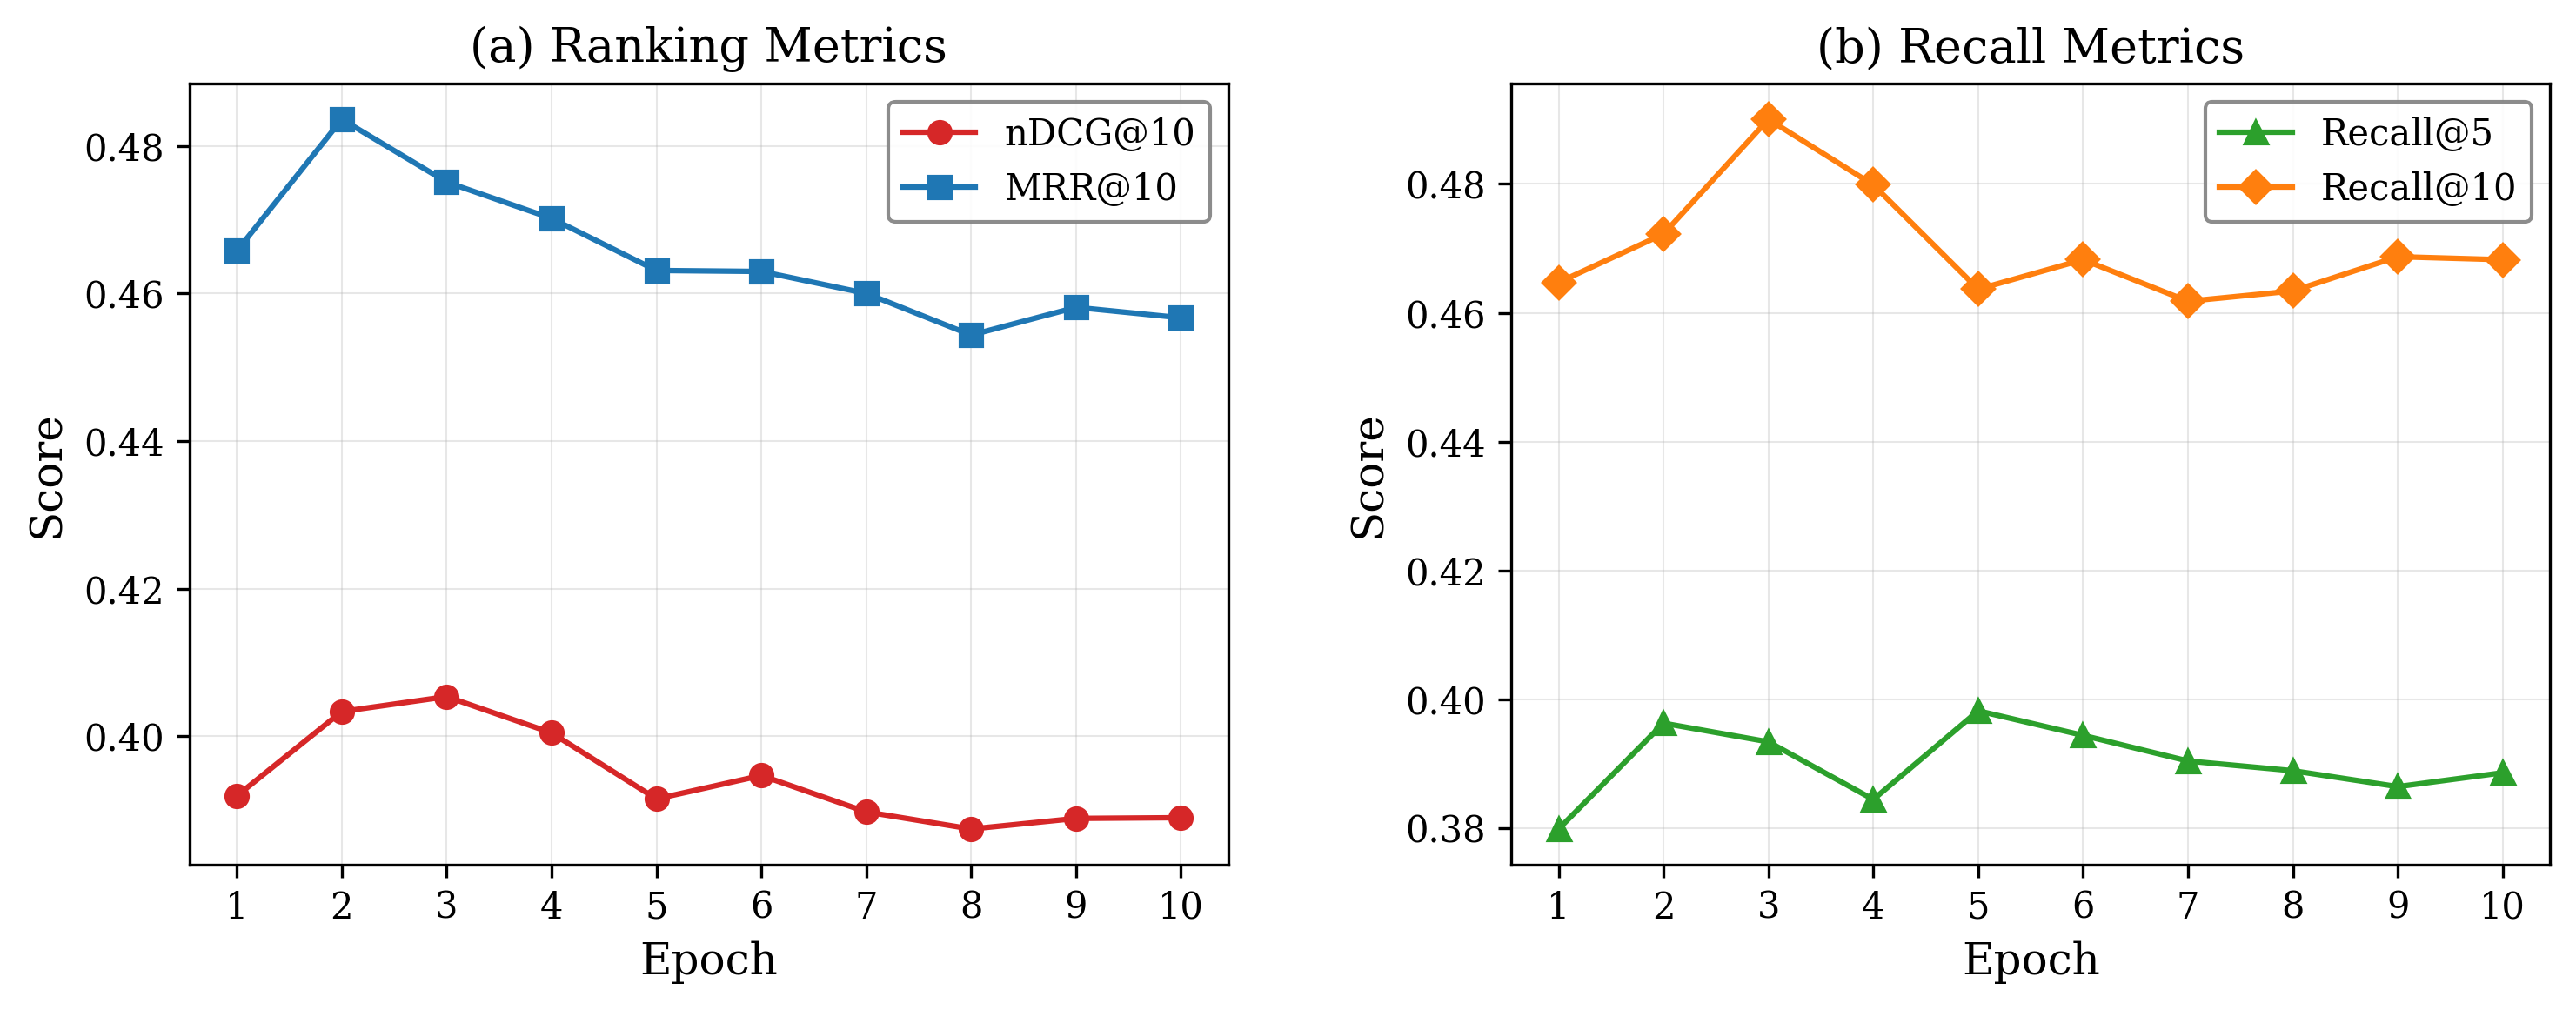
\includegraphics[width=\linewidth]{figures/training_curves.png}
        \footnotesize (a) \texttt{bge-small-en} (33M)
    \end{minipage}
    \hfill
    \begin{minipage}{0.49\linewidth}
        \centering
        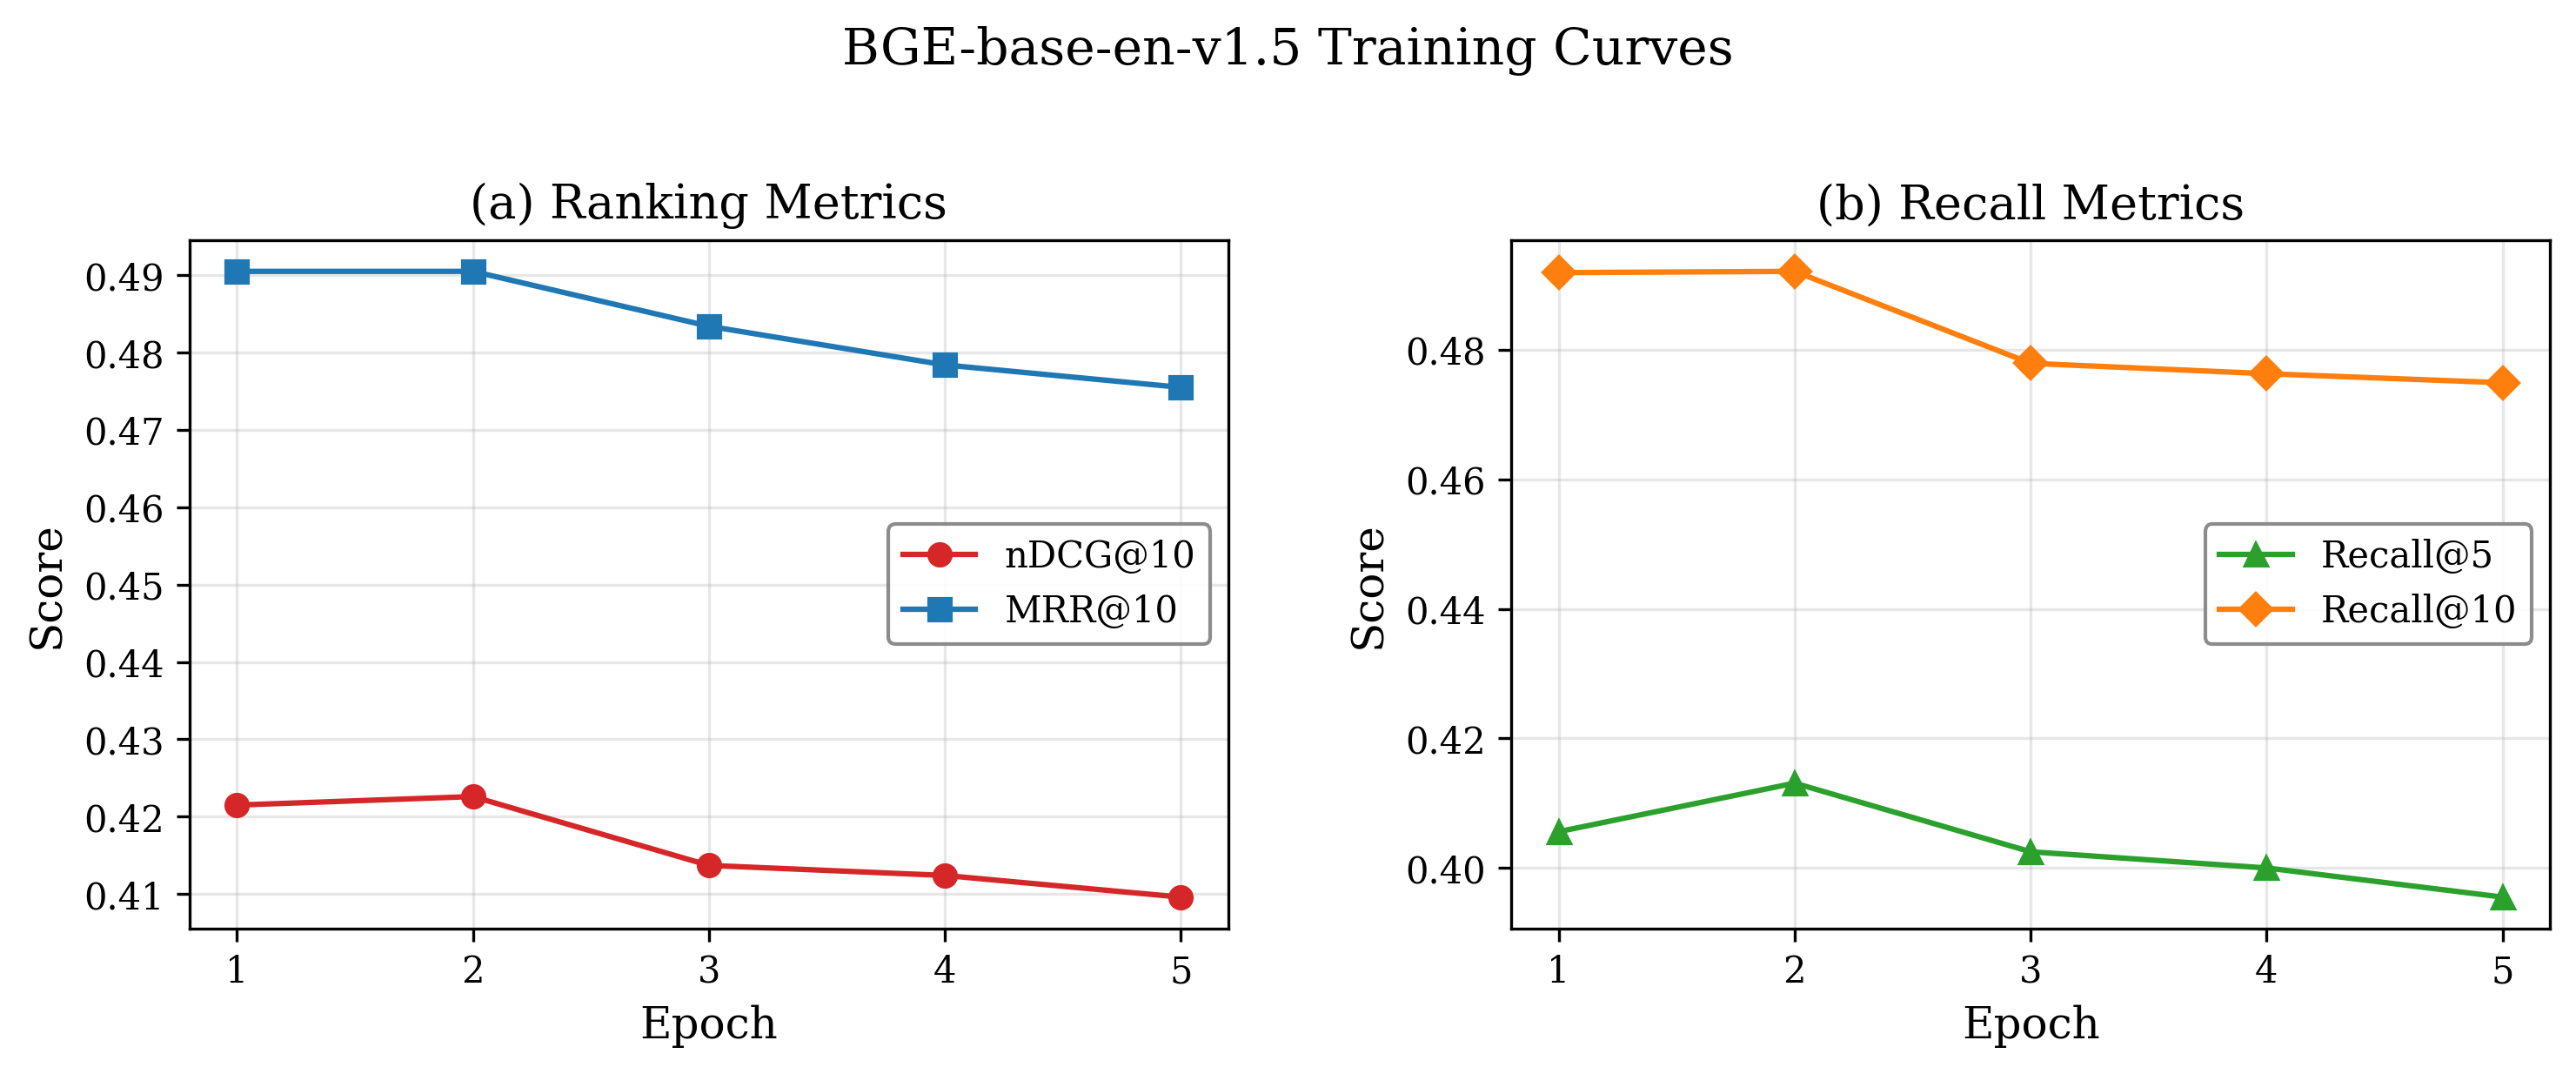
\includegraphics[width=\linewidth]{figures/training_curves_base_clean.png}
        \footnotesize (b) \texttt{bge-base-en-v1.5} (110M)
    \end{minipage}
    \caption{Validation metrics across training epochs. Both models peak early (epoch~2--3) and degrade with continued training, indicating that 14K training pairs cannot support extended fine-tuning without overfitting.}
    \label{fig:training_curves}
\end{figure}

\paragraph{Apparent improvement is recovery to zero-shot.}
A subtle but important observation: for \texttt{bge-base-en-v1.5}, epoch~1 dev nDCG@10 (0.4215) is actually \emph{below} the zero-shot baseline (0.4223), and the ``rise'' from epoch~1 to epoch~2 (0.4226) only brings the model back to its starting point.
Without an explicit zero-shot reference line, the curve gives the misleading impression that fine-tuning is helping.
This finding underscores the value of always evaluating zero-shot baselines for the same encoder when reporting fine-tuning gains.

\subsection{Scaling Trajectory and Embedding Space}

To inspect the geometry learned by fine-tuning, we project a random sample of fine-tuned query and document embeddings to two dimensions with t-SNE (Figure~\ref{fig:scaling_tsne}, right).
Queries do not form an isolated cluster; instead they are interleaved with the document points and concentrate in regions of high passage density, consistent with the cosine-similarity training objective shrinking the query--passage distribution gap that asymmetric retrieval models otherwise inherit from pretraining.
The visualization is qualitative and does not by itself imply higher retrieval accuracy, but it provides a sanity check that fine-tuning has reshaped the embedding space rather than merely rescaling distances.

\begin{figure}[t]
    \centering
    \begin{minipage}{0.49\linewidth}
        \centering
        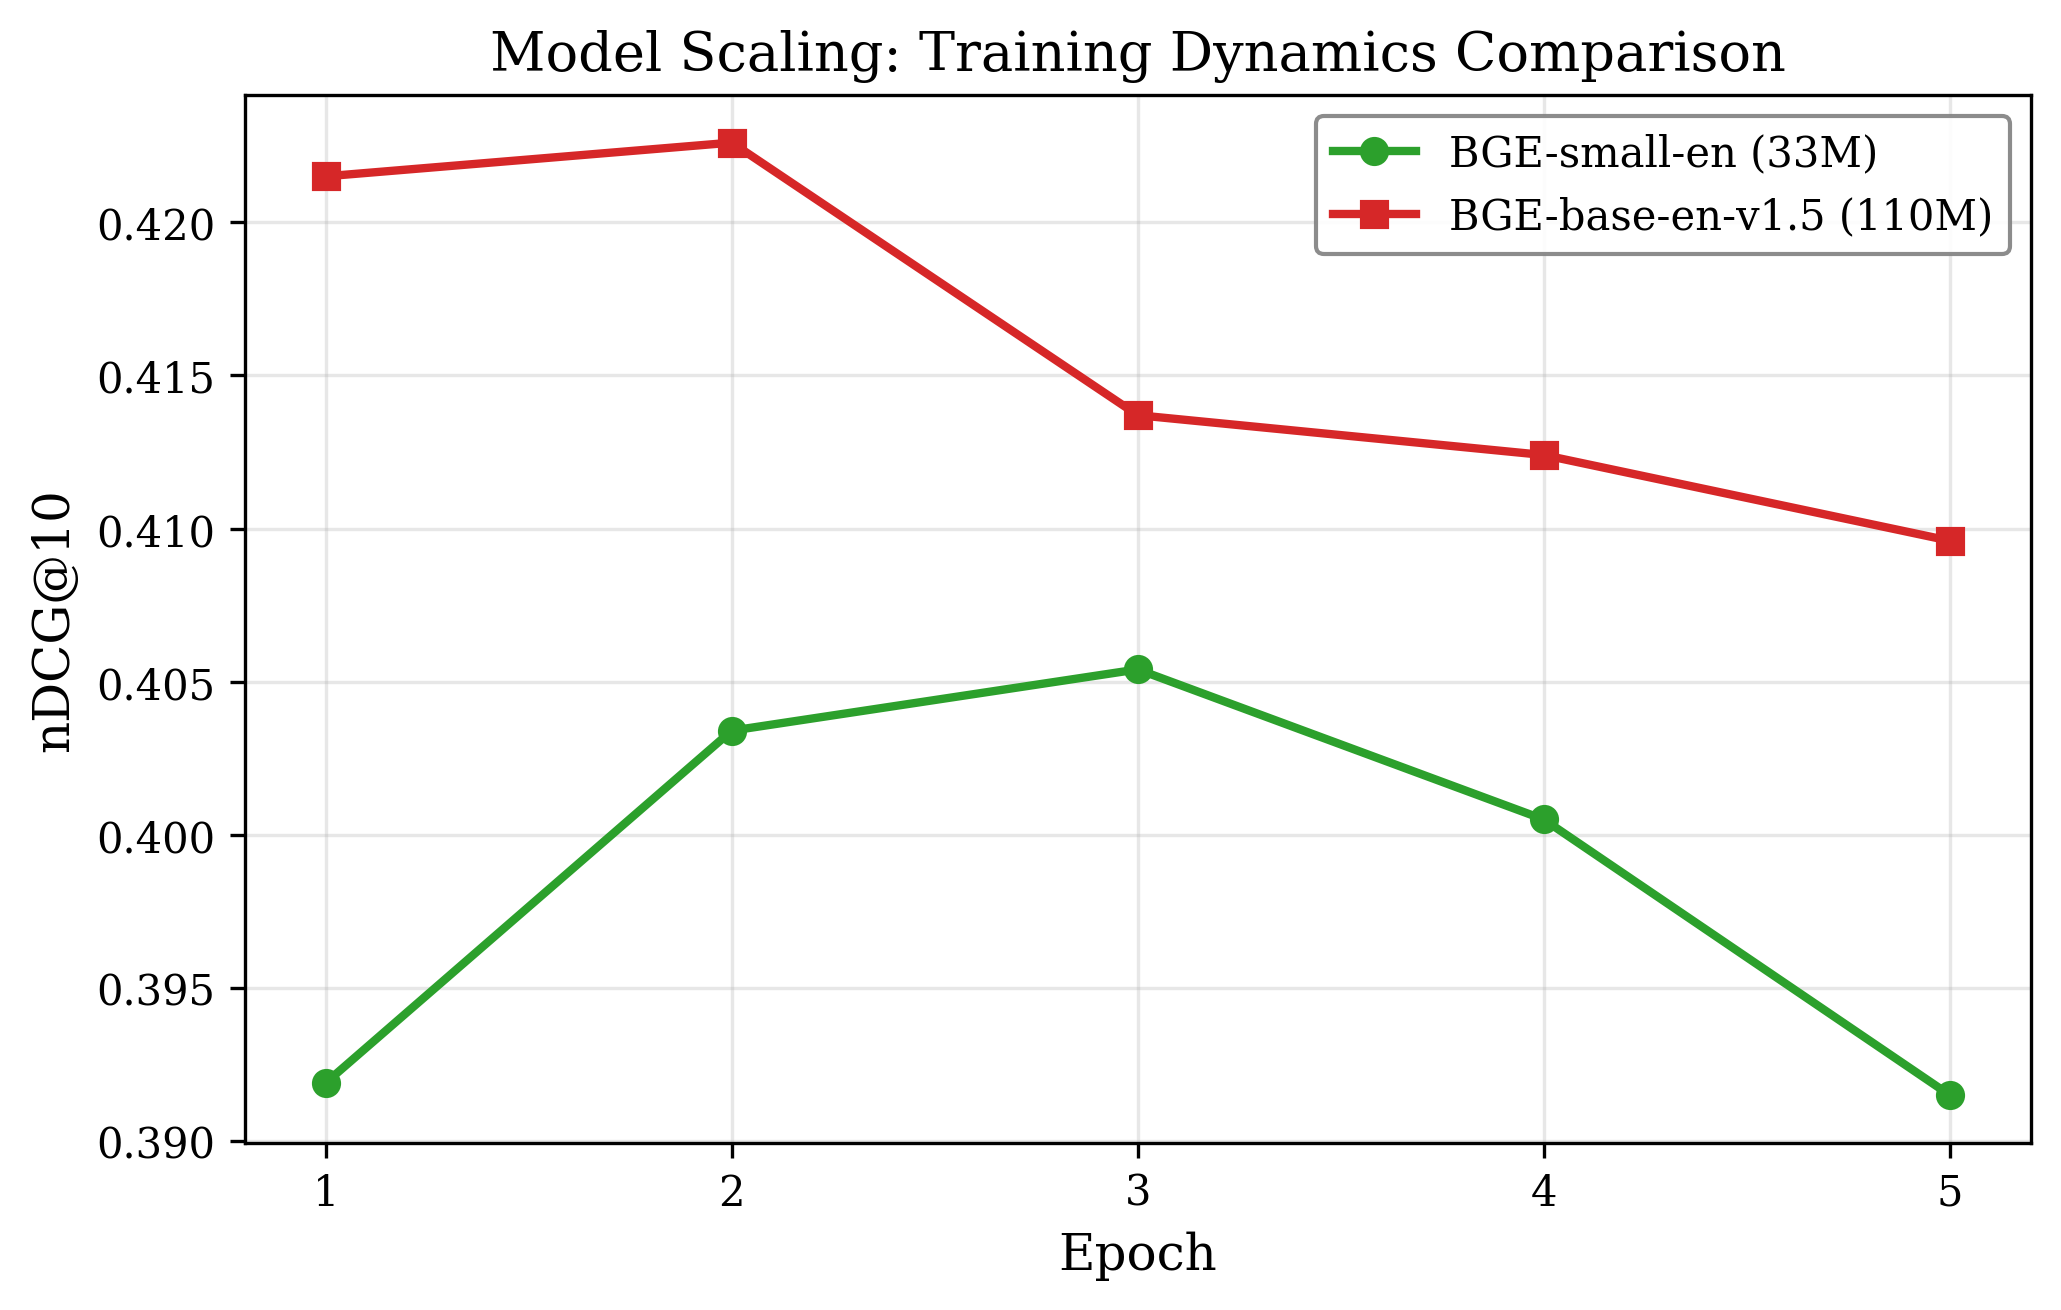
\includegraphics[width=\linewidth]{figures/scaling_comparison.png}
        \footnotesize (a) Model scaling trajectory
    \end{minipage}
    \hfill
    \begin{minipage}{0.49\linewidth}
        \centering
        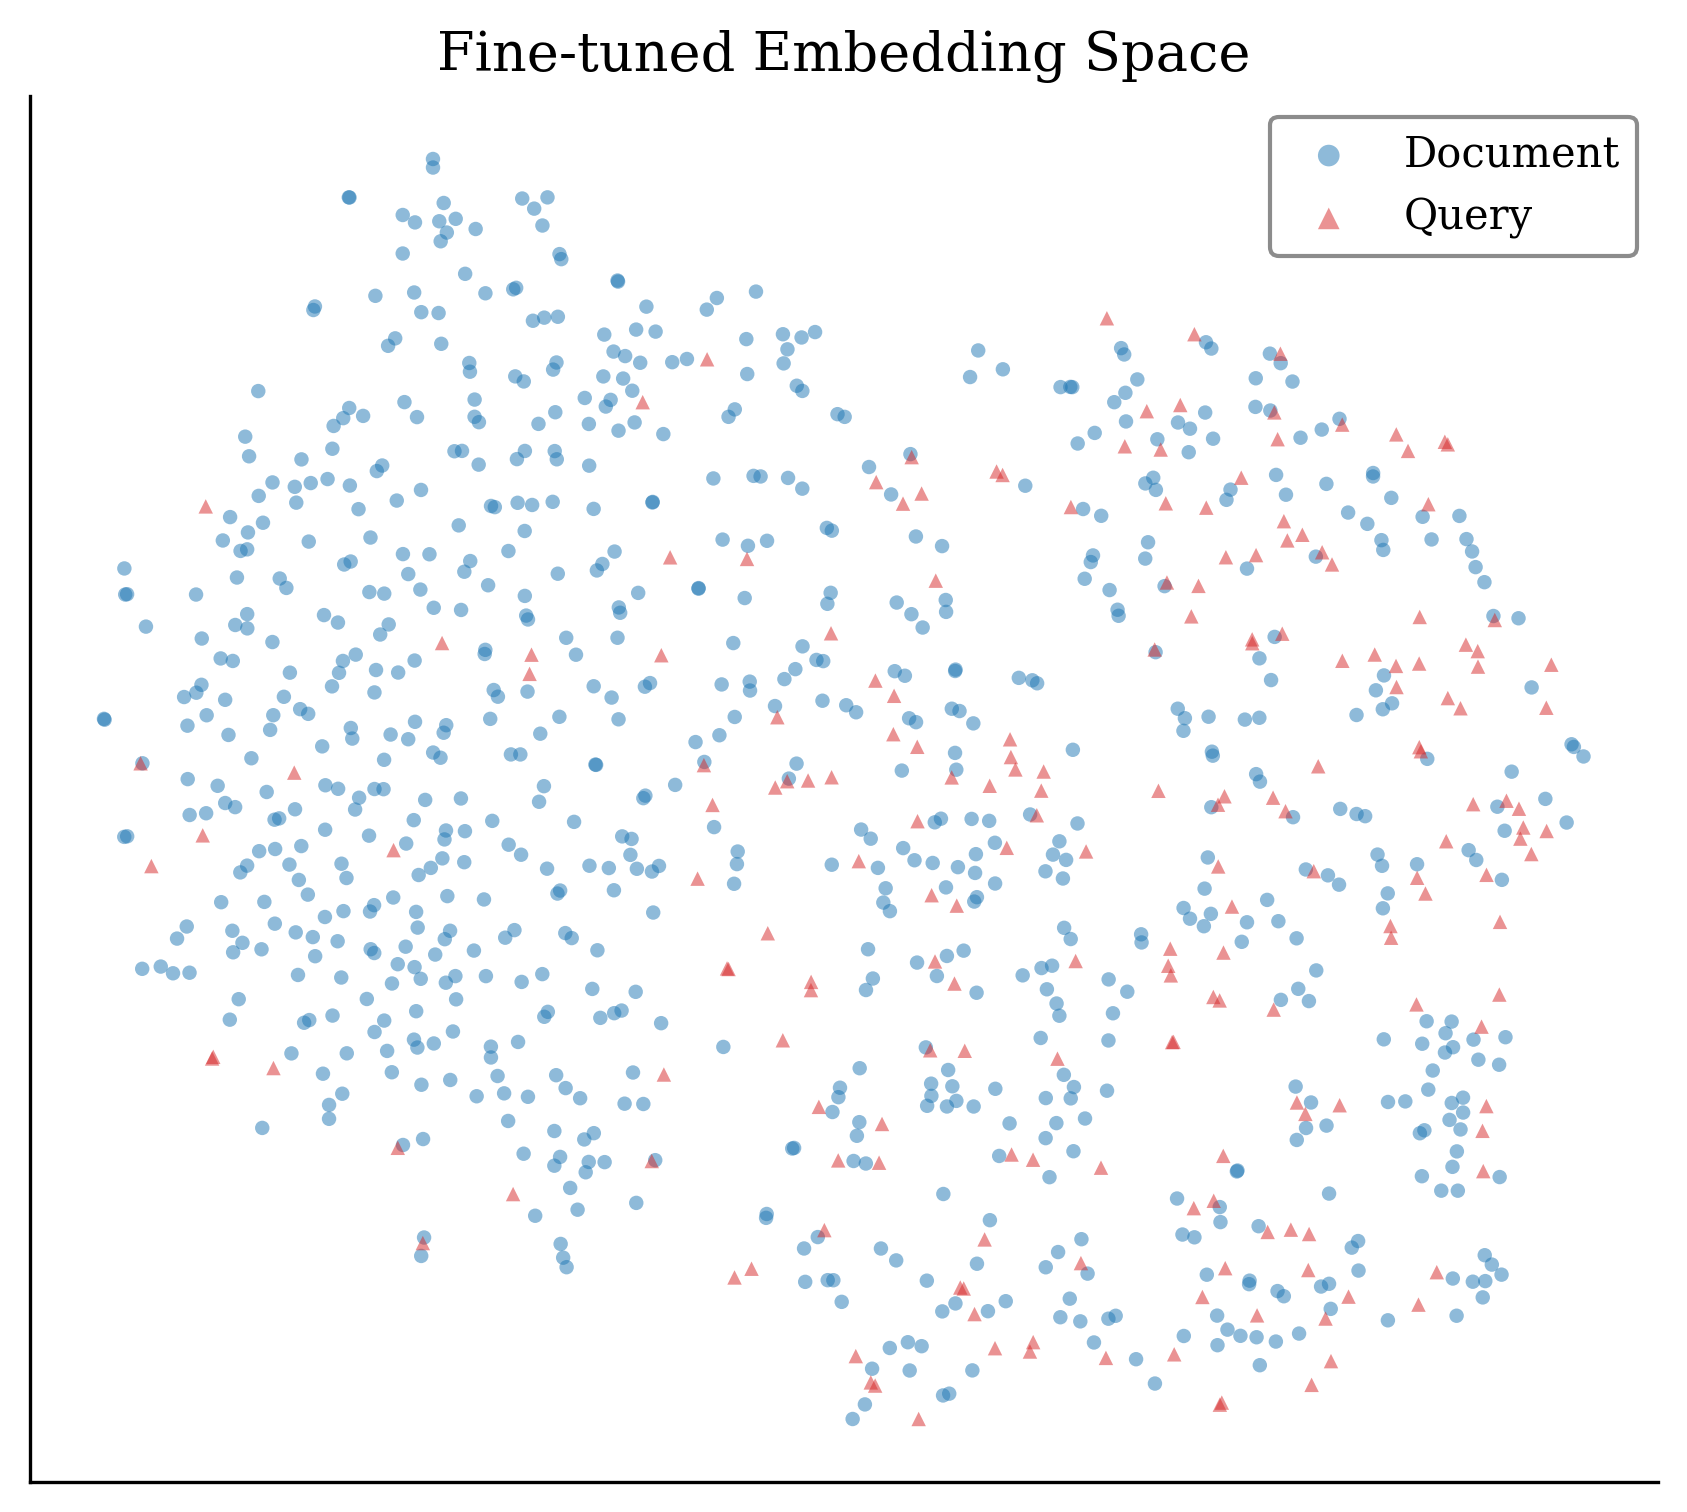
\includegraphics[width=0.85\linewidth]{figures/tsne_finetuned.png}
        \footnotesize (b) Fine-tuned embedding space (t-SNE)
    \end{minipage}
    \caption{(a) Validation nDCG@10 comparison between \texttt{bge-small-en} (33M) and \texttt{bge-base-en-v1.5} (110M) across training epochs; the larger model maintains a consistent advantage. (b) t-SNE projection of sampled query and document embeddings from the fine-tuned model; queries are interleaved with relevant document clusters rather than forming a separate cluster.}
    \label{fig:scaling_tsne}
\end{figure}

\subsection{Error Analysis}

We identify two systematic failure modes by inspecting top-10 retrieval results on queries where nDCG@10 falls below 0.1.

\textbf{Polysemy and domain ambiguity.}
For the query \emph{``How do I calculate my return on investment?''}, the model retrieves passages about tax return filing rather than ROI computation.
The term ``return'' is polysemous in finance, and the embedding model conflates distinct financial concepts that share surface-level similarity.
This pattern recurs for terms like ``margin'' (profit margin vs.\ margin trading) and ``option'' (stock option vs.\ choice).

\textbf{Numerical and conditional reasoning.}
For queries such as \emph{``What is the capital gains tax rate for income above \$100K?''}, the model retrieves passages discussing capital gains tax in general but fails to match the specific income threshold.
Embedding-based retrieval cannot perform arithmetic comparisons or conditional reasoning, so it treats all capital-gains-related passages as equally relevant regardless of numerical specifics.

These failures suggest that a cross-encoder reranker (which can attend jointly to query and passage tokens) or a hybrid BM25+dense approach could address cases where first-stage dense retrieval is insufficient.

\section{Conclusion}

\paragraph{Summary of findings.}
We studied domain-adaptive fine-tuning of pretrained BGE retrievers on financial text and observed a clear capacity-dependent pattern.
For the smaller \texttt{bge-small-en} (33M), fine-tuning lifts test nDCG@10 from 0.3109 to 0.3916 (+26.0\%), confirming H1.
For the stronger \texttt{bge-base-en-v1.5} (110M), the zero-shot baseline already reaches nDCG@10 of 0.4062 and fine-tuning provides no reliable improvement (0.4053, within measurement noise), a result robust across four hyperparameter configurations.
Hard negative mining without denoising further degrades performance on sparsely labeled data (H2 refuted).
Together, these results suggest that the value of small-scale domain fine-tuning depends on how well the pretrained encoder has already covered the target domain, and that practitioners should always benchmark against the same-encoder zero-shot baseline before claiming fine-tuning gains.

\paragraph{Limitations.}
Our study is limited to a single benchmark (FiQA) with sparse binary relevance labels.
The reversal we observe at the 110M scale may not extend to substantially larger encoders or to denser-labeled retrieval datasets.
We did not explore cross-encoder reranking or larger BGE variants (\texttt{bge-large-en-v1.5}, 335M).

\paragraph{Future work.}
Four directions follow from our findings:
(1) denoised hard negative mining (e.g., using a cross-encoder to filter false negatives before training) to address H2;
(2) data scaling experiments to identify the training-set size at which fine-tuning becomes beneficial for the base model, characterizing where the capacity-data trade-off flips;
(3) hybrid retrieval combining BM25 with dense retrieval for queries with strong lexical signals;
(4) evaluation on additional financial benchmarks (e.g., FinMTEB) to test whether the small-vs-base reversal generalizes beyond FiQA.

\section*{Team Contributions}

\begin{table}[h]
    \centering
    \scriptsize
    \begin{tabular}{lp{10cm}}
        \toprule
        Member & Contributions \\
        \midrule
        Hongbin Zhong & Model fine-tuning and optimization (query instruction prefix, hard negative mining, model scaling ablation), multi-GPU training infrastructure setup on Georgia Tech cluster, evaluation pipeline implementation, hyperparameter experiments and ablation studies, co-writing of Method and Experiments sections. \\
        \midrule
        Jiaqi Deng & Data preparation and preprocessing pipeline, BM25 and zero-shot dense baseline implementations, visualization and figure generation (training curves, t-SNE, comparison plots), literature review and related work section, co-writing of Introduction, Data, and Conclusion sections. \\
        \bottomrule
    \end{tabular}
\end{table}

\bibliography{iclr2025_conference}
\bibliographystyle{iclr2025_conference}

\end{document}
